\chapter{Trigonometry}

\section{Trigonometric Functions of Real Numbers}
In this chapter the three main trigonometric functions (sine, cosine and tangent) will be studied. \ They
will be viewed as functions of real numbers. \ This means that the domains of the functions are the real numbers.
\ In chapter 3 the same functions will be viewed as functions of angles. \ this
means that the domains of the functions will be angles. \ The trigonometric functions defined in these two ways
are identical and there is a simple rule connecting the domains. \ Why do we show you the two approaches? \ Trigonometry
will be used to solve a variety of problems and these can be divided into two groups, dynamic problems and static problems. \ When
dynamic problems (such as problems involving motion) are being solved (chapter 2) real numbers will be used. \ When
static problems (such as finding distances and angles for triangles) are being solved (chapter 3) angles will be used. 

\section{The Unit Circle}
In this session frequent reference will be made to the measurement of distances around the perimeter
of the unit circle. \ The unit circle is defined as a circle centre $\left (0 ,0\right )$ radius $1$. \ Its equation is $x^{2} +y^{2} =1$. \ In mathematics we are always on the lookout for patterns that make our calculations
easier. \ for instance, recently we discussed the circle $x^{2} +y^{2} =25$. (Circle centre $\left (0 ,0\right )$ radius $5$.) \ We found the point $\left (3 ,4\right )$ was on the circle ($3^{2} +4^{2} =5^{2}$). \ The unit circle also has some patterns that you should become familiar with. 

\subsubsection{Example}
Show $\left (\frac{\sqrt{2}}{2} ,\frac{\sqrt{2}}{2}\right )$ is on the unit circle. 

Because we are given
the coordinates of the point we are required to show that $x^{2} +y^{2} =1$. 

$x^{2} +y^{2} =\genfrac{(}{)}{}{}{\sqrt{2}}{2}^{2} +\genfrac{(}{)}{}{}{\sqrt{2}}{2}^{2} =\frac{2}{4} +\frac{2}{4} =\frac{1}{2} +\frac{1}{2} =1$ 

So $x^{2} +y^{2} =1$ proves that $\left (\frac{\sqrt{2}}{2} ,\frac{\sqrt{2}}{2}\right )$ lies on the unit circle. 

\subsubsection{Example}
Given $\left (\frac{1}{2} ,a\right )$ lies on the unit circle find $a$. 

Because we are told the point lies on the unit circle we substitute
\begin{eqnarray*}\genfrac{(}{)}{}{}{1}{2}^{2} +a^{2} &  = & 1 \\
\frac{1}{4} +a^{2} &  = & 1 \\
a^{2} &  = & 1 -\frac{1}{4} =\frac{3}{4} \\
a &  = &  \pm \sqrt{\frac{3}{4}} = \pm \frac{\sqrt{3}}{\sqrt{4}} = \pm \frac{\sqrt{3}}{2}\end{eqnarray*}

This means there are two possible solutions $\left (\frac{1}{2} ,\frac{\sqrt{3}}{2}\right )$ and $\left (\frac{1}{2} , -\frac{\sqrt{3}}{2}\right )$. \ A diagram will show
this to you. \ Notice the right angled triangle we can draw to produce the result. 


\subsection{Terminal Points}
An important skill we require in this section is to be able to connect the coordinates of a point on the unit circle with a length on the circumference
of the unit circle. \ For this we have a convention. \ \emph{All
distances are measured anticlockwise from the point }$\left (1 ,0\right )$. \ (The textbook uses
the word counterclockwise in place of anticlockwise. \ These words are used interchangeably.) \ In
the digital world of today these terms are not as widely used as they were when only analog clocks had been invented. \ We
find them convenient words to use because they explain precisely what we want to say. 

We let $t$ be the distance to a point on the unit circle from the point $\left (1 ,0\right )$. \ $t$ is a real number so distances that are measured in an anticlockwise direction are positive and distances measured in a clockwise
direction are negative. 

\textbf{Definition:} When you measure a distance of $t$ around the perimeter of the unit circle and arrive at a point $P (x ,y)$ the point $P (x ,y)$ is defined as a \emph{terminal point}. \ (See the diagram on p 410.) 

Some terminal points are easy to find provided you remember how to find the perimeter of the unit circle.
\begin{eqnarray*}\text{Perimeter} &  = & 2 \pi  r\text{\ \ \ but if}r =1 \\
 &  = & 2 \pi  \times 1 =2 \pi \end{eqnarray*}

This means that if you measure from $\left (1 ,0\right )$ right around the unit circle to the starting point $t =2 \pi $. \ So if $t =2 \pi $ the terminal point is $\left (1 ,0\right )$. 

\subsubsection{Example}
Find the coordinates of the terminal point when (a) $t =\pi $ (b) $t =5 \pi $ (c) $t =\frac{ -3 \pi }{2}$ 

Terminal points are obtained from a sketch of the situation. 

(a) $\left ( -1 ,0\right )$ (b) $\left ( -1 ,0\right )$ (c) $\left (0 ,1\right )$ 

There are other values we will \ use
that are more easily deduced once chapter 6 in the textbook has been completed. \ At this stage it is easier to
state these in a table and focus on using the values obtained to solve other related problems. 

We give the terminal point for $0$, $\frac{\pi }{6}$, $\frac{\pi }{4}$, $\frac{\pi }{3}$ and $\frac{\pi }{2}$. 


\begin{tabular}[c]{|r|l|l|l|l|l|}\hline
$t$  & $0$  & $\frac{\pi }{6}$  & $\frac{\pi }{4}$  & $\frac{\pi }{3}$  & $\frac{\pi }{2}$  \\
\hline
Terminal Point  & $\left (1 ,0\right )$  & $\left (\frac{\sqrt{3}}{2} ,\frac{1}{2}\right )$  & $\left (\frac{\sqrt{2}}{2} ,\frac{\sqrt{2}}{2}\right )$  & $\left (\frac{1}{2} ,\frac{\sqrt{3}}{2}\right )$  & $\left (0 ,1\right )$  \\
\hline
\end{tabular}

These will be given if required in a test. 

\subsubsection{Example}
Use the table to find the terminal points for (a) $t =\frac{5 \pi }{3}$ (b) $t =\frac{ -7 \pi }{6}$ 

(a) $\left (\frac{1}{2} ,\frac{ -\sqrt{3}}{2}\right )$ (b) $\left (\frac{ -\sqrt{3}}{2} ,\frac{1}{2}\right )$ 

Examples 3 and 4 pp 411-413 are about finding
terminal points. 

\subsection{Reference Numbers}
A useful way to connect the terminal point with the distance around the unit circle $t$ is to define a further quantity, the \emph{reference number} $\bar{t}$. \ However if you understand how to relate a particular value of $t$ with an appropriate value in the first quadrant to allow you to use the table then the need for the definition of a reference
number may be unnecessary. \ In this course we will tackle problems using the approach given in example 4 above
until the need to define the reference number is unavoidable. 

\subsection{Exercises}
Show that the point is on the unit circle. 


\begin{description}
\item [1.]   
%TCIMACRO{\TeXButton{Start Two Columns}{\columnsep =30pt
% \begin {multicols}{2}}}%
%BeginExpansion
\columnsep =30pt
\begin {multicols}{2}
%EndExpansion
 $\left (\frac{3}{5} ,\frac{4}{5}\right )$ 

\item [3.]
$\left ( -\frac{2}{3} , -\frac{\sqrt{5}}{3}\right )$ 
%TCIMACRO{\TeXButton{End Two Columns}{\end {multicols}}}%
%BeginExpansion
\end {multicols}
%EndExpansion
\end{description}

The point $P$ is on the unit circle. \ Find $P (x ,y)$ from the given information. 


\begin{description}
\item [5.] The $x$-coordinate of $P$ is $\frac{4}{5}$ and $P$ is in quadrant I. 

\item [7.] The
$y$-coordinate of of $P$ is $\frac{2}{3}$ and the $x$-coordinate is negative. 

\item [9.]
The $x$-coordinate of $P$ is $ -\sqrt{2}/3$ and $P$ is in quadrant III. \end{description}

Find the terminal point $P (x ,y)$ on the unit circle determined by the given value of $t$. 


\begin{description}
\item [13.]   
%TCIMACRO{\TeXButton{Start Two Columns}{\columnsep =30pt
% \begin {multicols}{2}}}%
%BeginExpansion
\columnsep =30pt
\begin {multicols}{2}
%EndExpansion
 $t =\frac{\pi }{2}$ 

\item [15.] $t =\frac{5 \pi }{6}$ 
%TCIMACRO{\TeXButton{End Two Columns}{\end {multicols}}}%
%BeginExpansion
\end {multicols}
%EndExpansion
 

\item [17.]
%TCIMACRO{\TeXButton{Start Two Columns}{\columnsep =30pt
% \begin {multicols}{2}}}%
%BeginExpansion
\columnsep =30pt
\begin {multicols}{2}
%EndExpansion
 $t = -\frac{\pi }{3}$ 

\item [19.] $t =\frac{2 \pi }{3}$ 
%TCIMACRO{\TeXButton{End Two Columns}{\end {multicols}}}%
%BeginExpansion
\end {multicols}
%EndExpansion
 

\item [21.]
$t = -\frac{3 \pi }{4}$ 

\item [23.] Suppose that the terminal
point determined by $t$ is the point $\left (\frac{3}{5} ,\frac{4}{5}\right )$ on the unit circle. \ Find
the terminal point determined by each of the following. 

\item [(a)]
%TCIMACRO{\TeXButton{Start Two Columns}{\columnsep =30pt
% \begin {multicols}{2}}}%
%BeginExpansion
\columnsep =30pt
\begin {multicols}{2}
%EndExpansion
 $\pi  -t$ 

\item [(b)] $ -t$ 
%TCIMACRO{\TeXButton{End Two Columns}{\end {multicols}}}%
%BeginExpansion
\end {multicols}
%EndExpansion
 

\item [(c)]
%TCIMACRO{\TeXButton{Start Two Columns}{\columnsep =30pt
% \begin {multicols}{2}}}%
%BeginExpansion
\columnsep =30pt
\begin {multicols}{2}
%EndExpansion
 $\pi  +t$ 

\item [(d)] $t -\pi $ 
%TCIMACRO{\TeXButton{End Two Columns}{\end {multicols}}}%
%BeginExpansion
\end {multicols}
%EndExpansion
 \end{description}


%TCIMACRO{\TeXButton{Start Two Columns}{\columnsep =30pt
% \begin {multicols}{2}}}%
%BeginExpansion
\columnsep =30pt
\begin {multicols}{2}
%EndExpansion
 


%TCIMACRO{\TeXButton{End Two Columns}{\end {multicols}}}%
%BeginExpansion
\end {multicols}
%EndExpansion

\section{The Trigonometric Functions of Real Numbers}
In this section we define sine, cosine and tangent based on $t$ as defined in section $7.1$. \ You need to be very careful to decide which quadrant the terminal point is in
so that the signs of the trigonometric functions are correct. 

\textbf{Definitions:} Given a real number $t$. \ If we move a distance $t$ around the unit circle starting at the point $\left (1 ,0\right )$ and we arrive at a point $P (x ,y)$ then $x =\cos  t$, $y =\sin  t$ and $\frac{y}{x} =\tan  t$ $\left (x \neq 0\right )$. 

A sketch will show the relationship between
$t$, $x$, and $y$. 

A fundamental relationship between sine, cosine and tangent comes from these definitions
\begin{equation*}\tan  t =\frac{\sin  t}{\cos  t}
\end{equation*}

We call this relationship an \emph{identity} because it is true for all values
of $t$. 

There are six trigonometric functions. \ The other three are
secant, cosecant and cotangent. \ The are sometimes referred to as the reciprocal functions because: 

Secant is defined by $\sec  t =\frac{1}{\cos  t} =\frac{1}{x}$ 

Cosecant is defined by co$\sec  t =\frac{1}{\sin  t} =\frac{1}{y}$ ($ =$csc $t$) 

Cotangent is defined by $\cot  t =\frac{1}{\tan  t} =\frac{x}{y}$ $\left (y \neq 0\right )$ 

In this course we will focus on sine, cosine
and tangent and only use secant, cosecant and cotangent when it is unavoidable. 

The table in section 7.1 can now be extended to include
sine, cosine and tangent. 

\qquad \qquad
\begin{tabular}[c]{|c|c|c|c|c|}\hline
$t$  & Terminal Point  & $x =\cos  t$  & $y =\sin  t$  & $\frac{y}{x} =\tan  t$  \\
\hline
$0$  & $\left (1 ,0\right )$  & $1$  & $0$  & $\frac{0}{1} =0$  \\
\hline
$\frac{\pi }{6}$  & $\left (\frac{\sqrt{3}}{2} ,\frac{1}{2}\right )$  & $\frac{\sqrt{3}}{2}$  & $\frac{1}{2}$  & $\frac{1}{2} \div \frac{\sqrt{3}}{2} =\frac{1}{2} \times \frac{2}{\sqrt{3}} =\frac{1}{\sqrt{3}} =\frac{\sqrt{3}}{3}$  \\
\hline
$\frac{\pi }{4}$  & $\left (\frac{\sqrt{2}}{2} ,\frac{\sqrt{2}}{2}\right )$  & $\frac{\sqrt{2}}{2}$  & $\frac{\sqrt{2}}{2}$  & $\frac{\sqrt{2}}{2} \div \frac{\sqrt{2}}{2} =1$  \\
\hline
$\frac{\pi }{3}$  & $\left (\frac{1}{2} ,\frac{\sqrt{3}}{2}\right )$  & $\frac{1}{2}$  & $\frac{\sqrt{3}}{2}$  & $\frac{\sqrt{3}}{2} \div \frac{1}{2} =\frac{\sqrt{3}}{2} \times \frac{2}{1} =\sqrt{3}$  \\
\hline
$\frac{\pi }{2}$  & $\left (0 ,1\right )$  & $0$  & $1$  & $\frac{1}{0}$ undefined $\left ( =\infty \right )$  \\
\hline
\end{tabular}

Should you be asked about secant, cosecant or cotangent you should look up the respective reciprocal relationship and calculate it from that.


\subsubsection{Values of Trigonometric Functions}
The value of a trigonometric function consists of two parts the numerical part and the sign. \ you
must get both parts correct. \ In the previous section (example 4) you related the values of a terminal point
to another point in the first quadrant. \ A point on the unit circle could be in any one of the four quadrants.
\ You should develop an intuitive understanding of how this allows you to be sure of the sign of your answer.


\qquad \qquad \qquad \qquad
\begin{tabular}[c]{|c|c|c|c|c|c|}\hline
Quadrant  & $x$-coordinate  & $y$-coordinate  & $\cos $  & $\sin $  & $\tan $  \\
\hline
$1$  & $ +$  & $ +$  & $ +$  & $ +$  & $ +$  \\
\hline
$2$  & $ -$  & $ +$  & $ -$  & $ +$  & $ -$  \\
\hline
$3$  & $ -$  & $ -$  & $ -$  & $ -$  & $ +$  \\
\hline
$4$  & $ +$  & $ -$  & $ +$  & $ -$  & $ -$  \\
\hline
\end{tabular}

Some people learn this as a mnemonic All sin tan cos. (Meaning all are positive in the first quadrant, only sine is positive in the second quadrant,
only tangent is positive in the third quadrant and only cosine is positive in the fourth quadrant.) \ Two little
sentences that are sometimes seen to help you to get this right are "\textbf{A}ll \textbf{s}tudents \textbf{t}ake \textbf{c}alculus," and
"\textbf{ACTS} clockwise." This means that as soon as you know which quadrant the terminal point is in you know the sign of the trigonometric function.


These types of problems will be in two categories 


\begin{enumerate}
\item Problems where $t$ is a multiple of $\frac{\pi }{6}$ or $\frac{\pi }{4}$ 

\item Problems where $t$ is not a multiple of $\frac{\pi }{6}$ or $\frac{\pi }{4}$ 

\item Our special values of $t$, $0$, $\frac{\pi }{6}$, $\frac{\pi }{4}$, $\frac{\pi }{3}$, $\frac{\pi }{2}$ are all multiple of $\frac{\pi }{6}$ or $\frac{\pi }{4}$. \ They are all in the first quadrant and lead to our being able to relate our problem back
to these. \ when you are asked a question where the value of $t$ is a multiple of a special value of $t$ you are being tested on your ability to relate the question to the value for the special value so you should ensure you have
answered it to show this. (A calculator answer is not appropriate for these questions.) 

\item When
$t$ is not one of these special values you should use your calculator set in \emph{radians} mode. \end{enumerate}


\subsubsection{Example}
\begin{description}
\item [(a)] $\tan  \frac{3 \pi }{4} = -1$ 

\item [(b)] $\sin  \genfrac{(}{)}{}{}{ -7 \pi }{3} =\frac{ -\sqrt{3}}{2}$ 

\item [(c)] $\cos  -2.1 = -0.5048$ (4 dp) \end{description}


\subsection{Even and Odd Functions}
Even functions have the $y$-axis as an axis of symmetry. \\\relax Odd functions have point symmetry about
the origin. 

For even functions $f (x) =f ( -x)$ which is the same as saying $f ( -x) =f (x)$. \\\relax For odd functions $f (x) = -f ( -x)$ which is the same as saying $f ( -x) = -f (x)$. 

When we talk about odd and even functions these ideas keep recurring. \ Sine,
cosine and tangent can be looked at from this perspective too. \ Regardless of the quadrant for the terminal point
$\sin  t = -\sin  t$ so sine is an odd function. \ A diagram shows this. \ Also
$\cos  t =\cos  ( -t)$ so cosine is an even function. \ The same diagram shows this 

For the
tangent function
\begin{equation*}\tan  ( -t) =\frac{\sin  ( -t)}{\cos  ( -t)} =\frac{ -\sin  t}{\cos  t} = -\tan  t
\end{equation*}

So tangent is also an odd function. 

This subject will be explored further in
the next section. 

\subsection{The Fundamental Pythagorean Identity}
The unit circle has equation $x^{2} +y^{2} =1$ and we define $x =\cos  t$ and $y =\sin  t$ so
\begin{equation*}x^{2} +y^{2} =1 \leadsto \left (\cos  t\right )^{2} +\left (\sin  t\right )^{2} =1
\end{equation*}

This is always written
\begin{equation*}\sin ^{2} t +\cos ^{2} t =1
\end{equation*}

This is an \emph{identity} which means it is true for all values of $t$. 

Whereas the textbook gives eight fundamental identities on p 424 we will restrict our list to the two
previously mentioned, namely $\tan  t =\frac{\sin  t}{\cos  t}$ and $\sin ^{2} t +\cos ^{2} t =1$, and only use the other six when it is unavoidable. 

\subsection{Exercises}
Give the exact value of the trigonometric function
at the given real number 


\begin{tabular}[c]{rllllllrlllll}3.\vspace*{0.25cm}
& (a)  & $\sin  \left ( -\frac{\pi }{3}\right )$  &  & (b)  & $\cos  \left ( -\frac{\pi }{3}\right )$  &  & 5.  & (a)
& $\cos  \pi $  &  & (b)  & $\cos  \left ( -\pi \right )$  \\
7.\vspace*{0.25cm}  & (a)
& $\sin  \frac{\pi }{2}$  &  & (b)  & $\sin  \frac{3 \pi }{2}$  &  & 9.  & (a)
& $\cos  \frac{\pi }{2}$  &  & (b)  & $\cos  \frac{5 \pi }{2}$  \\
13.\vspace*{0.25cm}  & (a)
& $\cos  \frac{\pi }{3}$  &  & (b)  & $\cos  \left ( -\frac{\pi }{3}\right )$  &  & 15.  & (a)
& $\tan  \frac{\pi }{6}$  &  & (b)  & $\tan  \left ( -\frac{\pi }{6}\right )$
\end{tabular}

The terminal point $P (x ,y)$ determined bt t is given. \ Find $\sin  t$, $\cos  t$ and $\tan  t\text{.}$ 


\begin{tabular}[c]{lllllllllll}27.  & $\left (\frac{3}{5} ,\frac{4}{5}\right )$  & \ \ \ \ \ \ \ \ \ \ \ \ \ \ \ \ \ \ \ \ \ \ \ \ \ \ \ \  &  &  &  &  &  & 29.
& $\left (\frac{\sqrt{5}}{4} , -\frac{\sqrt{11}}{4}\right )$  & 
\end{tabular}

Find the approximate value of the trigonometric function using the calculator. 

\begin{tabular}[c]{lllllllllll}35.  & $\sin  1$  & \ \ \ \ \ \  & 37.
& $\sin  1.2$  & \ \ \ \ \ \  & 39.
& $\tan  0.8$  & \ \ \ \ \ \  & 41.
& $\cos  4.1$
\end{tabular}



\section{Trigonometric Graphs - Sine and Cosine}

\subsection{Graphs of the Sine and Cosine Functions}
You should be familiar with the fundamental graphs of $y =\sin  t$ and $y =\cos  t$. \ These graphs are the basis of this section. \ Omnigraph
can easily show you the shape of $y =\sin  t$ and $y =\cos  t$ so if you are asked to draw a rough sketch of these curves you should plot a few key points and draw a smooth curve between them. \ You
will usually be given the required domain however if you are not you would choose to draw these for one complete cycle ($0 -2 \pi $). \ To sketch $y =\sin  t$ it is enough to select as key points $t =0$, $\frac{\pi }{2}$, $\pi $, $\frac{3 \pi }{2}$, $2 \pi $. 


\begin{tabular}[c]{|l|l|l|l|l|l|}\hline
$t$  & $0$  & $\frac{\pi }{2}$  & $\pi $  & $\frac{3 \pi }{2}$  & $2 \pi $  \\
\hline
$y =\sin  t$  & $0$  & $1$  & $0$  & $ -1$  & $0$  \\
\hline
\end{tabular}

Similarly to sketch $y =\cos  t$ the same values of $t$ give 


\begin{tabular}[c]{|l|l|l|l|l|l|}\hline
$t$  & $0$  & $\frac{\pi }{2}$  & $\pi $  & $\frac{3 \pi }{2}$  & $2 \pi $  \\
\hline
$y =\cos  t$  & $1$  & $0$  & $ -1$  & $0$  & $1$  \\
\hline
\end{tabular}

You will be aware that these curves repeat this pattern every $2 \pi $ where $t$ extends in both the positive and negative directions. 

$0 -2 \pi $ represents one complete cycle. \ Mathematically we say
\begin{eqnarray*}\sin  \left (t +2 n \pi \right ) &  = & \sin  t\text{\ \ \ for any integer}n \\
\cos  \left (t +2 n \pi \right ) &  = & \cos  t\text{\ \ \ for any integer}n\end{eqnarray*}

Aside: instead of "for any integer $n$" we can write $ \forall n \in \mathbb{Z}$. 

A function that displays this characteristic is described as \emph{periodic} and for $y =\sin  t$ and $y =\cos  t$ the \emph{period} is $2 \pi $. 

You will often be asked to state the period of a trigonometric function so for sine and cosine it
is wise to remember that often the period is $2 \pi $. \ This means you need only worry about the distinctly different class of examples
of sine and cosine where the period is not $2 \pi $. 

You will sometimes be asked to sketch a graph for a given number of periods or a given number of cycles. These are two different ways of saying the same thing. 

\subsection{The Transformations of Sine and Cosine}
The six transformations we meet in this course are applied to sine and cosine. 

\begin{enumerate}
\item Vertical shift 
\item Horizontal shift 
\item Vertical stretch 
\item Horizontal stretch 
\item Reflection in the $x$-axis 
\item Reflection in the $y$-axis 
\end{enumerate}

We adopt four approaches to tackle these problems 

\begin{enumerate}
\item Describe the transformation in words. 
\item Rough sketch based on transformations. 
\item Rough sketch based on substitution. 
\item Omnigraph
graph. 
\end{enumerate}


\subsubsection{Example}
Sketch $y =\sin  \left (t -\frac{\pi }{2}\right ) +3$ 

1. This may be considered as a sine curve shifted $\frac{\pi }{2}$ to the right and $3$ upwards. 

\textbf{Definition:} A horizontal shift of a sine curve or cosine curve is called a \emph{phase
shift}. 

2. Transform the 5 point summary 


\begin{tabular}[c]{|l|l|l|l|l|l|}\hline
$t$  & $0$  & $\frac{\pi }{2}$  & $\pi $  & $\frac{3 \pi }{2}$  & $2 \pi $  \\
\hline
$\sin  t$  & $0$  & $1$  & $0$  & $ -1$  & $0$  \\
\hline
$\sin  \left (t -\frac{\pi }{2}\right )$  & $ -1$  & $0$  & $1$  & $0$  & $ -1$  \\
\hline
$\sin  \left (t -\frac{\pi }{2}\right ) +3$  & $2$  & $3$  & $4$  & $3$  & $2$  \\
\hline
\end{tabular}

You would sketch this if required 

3. The difference between this approach and the previous one is that the values are calculated
from the 5 values of $t$. \ Maybe an additional row containing $t -\frac{\pi }{2}$ values will help. 


\begin{tabular}[c]{|l|l|l|l|l|l|}\hline
$t$  & $0$  & $\frac{\pi }{2}$  & $\pi $  & $\frac{3 \pi }{2}$  & $2 \pi $  \\
\hline
$t -\frac{\pi }{2}$  & $ -\frac{\pi }{2}$  & $0$  & $\frac{\pi }{2}$  & $\pi $  & $\frac{3 \pi }{2}$  \\
\hline
$\sin  \left (t -\frac{\pi }{2}\right ) +3$  & $2$  & $3$  & $4$  & $3$  & $2$  \\
\hline
\end{tabular}

You would sketch this if required. 

4. Omnigraph confirms this 

   
\setlength\fboxrule{0.01in}\setlength\fboxsep{0.2in}\fcolorbox[HTML]{000000}{FFFFFF}{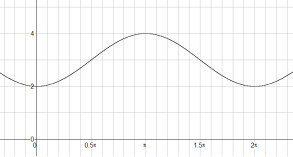
\includegraphics[ width=4.427in, height=2.3886in,]{L4SZ270G}
}


You would select the most appropriate way to tackle a problem based on the information given and the outcome expected. 

\subsubsection{Example}
Sketch $y =\cos  (x -\frac{\pi }{6})$ 

You could use a table of values however this is $y =\cos  x$ with a horizontal shift of $\frac{\pi }{6}$ to the right. 

Complete the following to show the answer. (This is the graph of $y =\cos  x .)$ 

   
\setlength\fboxrule{0.01in}\setlength\fboxsep{0.2in}\fcolorbox[HTML]{000000}{FFFFFF}{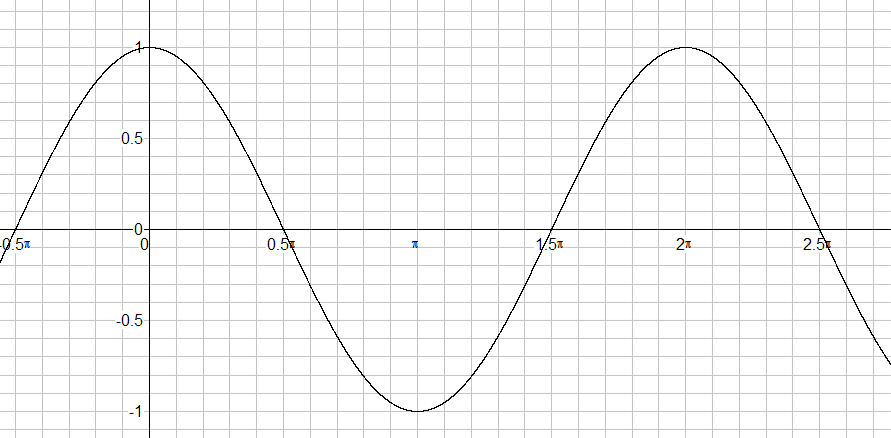
\includegraphics[ width=4.9095in, height=2.4275in,]{L4SZ270H}
}


\subsubsection{Example}
Sketch $y =2 \cos  t$ 


\begin{tabular}[c]{|l|l|l|l|l|l|}\hline
$t$  & $0$  & $\frac{\pi }{2}$  & $\pi $  & $\frac{3 \pi }{2}$  & $2 \pi $  \\
\hline
$\cos  t$  & $1$  & $0$  & $ -1$  & $0$  & $1$  \\
\hline
$2 \cos  t$  & $2$  & $0$  & $ -2$  & $0$  & $2$  \\
\hline
\end{tabular}

This is a vertical stretch of 2. \ You could roughly sketch this or use Omnigraph. 


\setlength\fboxrule{0.01in}\setlength\fboxsep{0.2in}\fcolorbox[HTML]{000000}{FFFFFF}{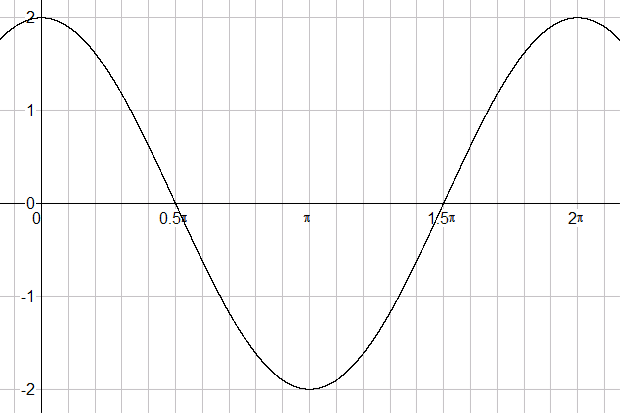
\includegraphics[ width=3.09in, height=2.0669in,]{L4SZ270I}
}


In general $y =a \sin  x$ represents a vertical stretch of $y =\sin  x$ by $a$. \ If $a$ is negative the transformation can either be described as a negative stretch or (preferably) as a \emph{stretch}
of $\left \vert a\right \vert $ followed by a \emph{reflection} in the $x$-axis. \ Recall the reflection of $y =f \left (x\right )$ in the $x$-axis is $y = -f \left (x\right )$. \ The number $\left \vert a\right \vert $ is called the \emph{amplitude} for both $y =\sin  x$ and $y =\cos  x\text{.}$ 

If $0 <a <1$ the fractional stretch causes the curve to shrink vertically. \ For instance the curve
$y =\sin  x$ has a maximum value of $1$ and a minimum value of $ -1$. \ the curve $y =\frac{1}{2} \sin  x$ has a maximum value of $\frac{1}{2}$ and a minimum value of $ -\frac{1}{2}$. 

\subsubsection{Example}
Sketch $y =\cos  ( -t)\text{.}$ 

Recall the reflection of $y =f (x)$in the $y$-axis is $y =f ( -x)$ so you would expect $y =\cos  ( -t)$ to be the reflection of $y =\cos  t$ in the $y$-axis. 


\begin{tabular}[c]{|l|l|l|l|l|l|lllllll}
$t$  & $0$  & $\frac{\pi }{2}$  & $\pi $  & $\frac{3 \pi }{2}$  & $2 \pi $  &  & $t$  & $0$  & $\frac{\pi }{2}$  & $\pi $  & $\frac{3 \pi }{2}$  & $2 \pi $  \\
 $ -t$  & $0$  & $ -\frac{\pi }{2}$  & $ -\pi $  & $ -\frac{3 \pi }{2}$  & $ -2 \pi $  &  & $\cos  t$  & $1$  & $0$  & $ -1$  & $0$  & $1$  \\
 $\cos  \left ( -t\right )$  & $1$  & $0$  & $ -1$  & $0$  & $1$  &  &  &  &  &  &  &  \\
\multicolumn{1}{|l}{
}
\end{tabular}

You can see from the table at the right that this looks exactly the same as
$y =\cos  t$ so $\cos  t$ is an \emph{even} function. \ When the $y$-axis is an axis of symmetry the function is an \emph{even} function. 

   
\setlength\fboxrule{0.01in}\setlength\fboxsep{0.2in}\fcolorbox[HTML]{000000}{FFFFFF}{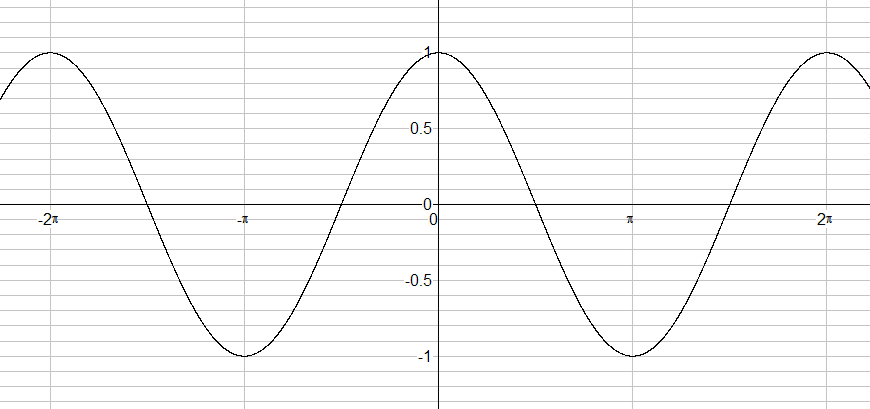
\includegraphics[ width=4.587in, height=2.1689in,]{L4SZ270J}
}


\subsubsection{Example}
Sketch $y =\sin  \frac{1}{2} x$ 


\begin{tabular}[c]{|l|l|l|l|l|l|l|l|l|l|}\hline
$x$  & $0$  & $\frac{\pi }{2}$  & $\pi $  & $\frac{3 \pi }{2}$  & $2 \pi $  & $\frac{5 \pi }{2}$  & $3 \pi $  & $\frac{7 \pi }{2}$  & $4 \pi $  \\
\hline
$\frac{1}{2} x$  & $0$  & $\frac{\pi }{4}$  & $\frac{\pi }{2}$  & $\frac{3 \pi }{4}$  & $\pi $  & $\frac{5 \pi }{4}$  & $\frac{3 \pi }{2}$  & $\frac{7 \pi }{4}$  & $2 \pi $  \\
\hline
$\sin  \frac{1}{2} x$  & $0$  &  & $1$  &  & $0$  &  & $ -1$  &  & $0$  \\
\hline
\end{tabular}

In this case one cycle is achieved only after $x$ has reached $4 \pi $. \ The period therefore is $4 \pi $. 

   
\setlength\fboxrule{0.01in}\setlength\fboxsep{0.2in}\fcolorbox[HTML]{000000}{FFFFFF}{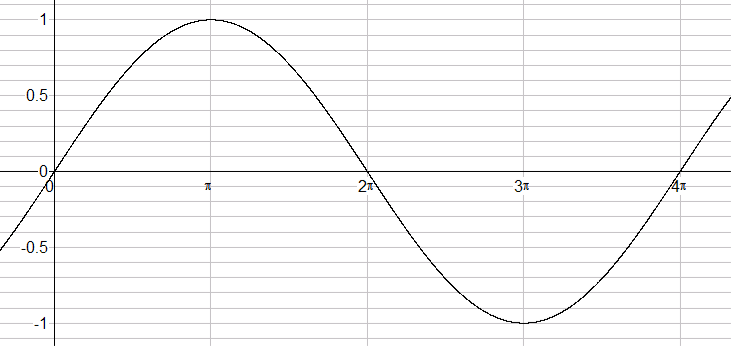
\includegraphics[ width=4.0698in, height=1.9372in,]{L4SZ270K}
}


\subsubsection{Example}
Sketch $y =\cos  2 x$ 


\begin{tabular}[c]{|l|l|l|l|l|l|}\hline
$x$  & $0$  & $\frac{\pi }{2}$  & $\pi $  & $\frac{3 \pi }{2}$  & $2 \pi $  \\
\hline
$2 x$  & $0$  & $\pi $  & $2 \pi $  & $3 \pi $  & $4 \pi $  \\
\hline
$\cos  2 x$  & $1$  & $ -1$  & $1$  & $ -1$  & $1$  \\
\hline
\end{tabular}

Maybe this is enough to enable you to sketch the curve. \ You notice the zeros that you usually get
in the table are missing and the way to include them is to select intermediate $x$ values. 


\begin{tabular}[c]{|l|l|l|l|l|l|}\hline
$x$  & $0$  & $\frac{\pi }{4}$  & $\frac{\pi }{2}$  & $\frac{3 \pi }{4}$  & $\pi $  \\
\hline
$2 x$  & $0$  & $\frac{\pi }{2}$  & $\pi $  & $\frac{3 \pi }{2}$  & $2 \pi $  \\
\hline
$\cos  2 x$  & $1$  & $0$  & $ -1$  & $0$  & $1$  \\
\hline
\end{tabular}

   
\setlength\fboxrule{0.01in}\setlength\fboxsep{0.2in}\fcolorbox[HTML]{000000}{FFFFFF}{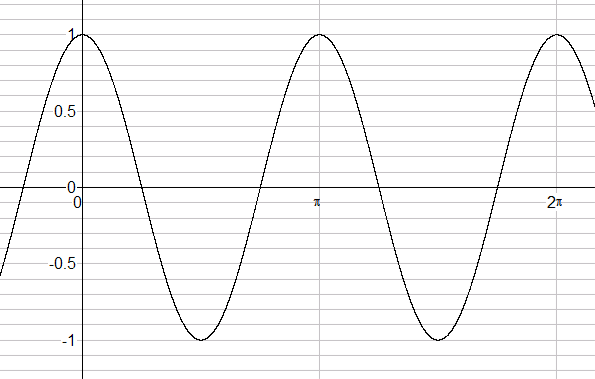
\includegraphics[ width=3.0666in, height=1.9614in,]{L4SZ270L}
}


Notice by sketching from $0$ to $2 \pi $ $2$ cycles are drawn. \ The period here is $\pi $. \ There is a pattern emerging. \ Given
$y =\sin  k x$ or $y =\cos  k x$. \ The value of $k$ tells you how many cycles in $2 \pi $. \ If $k =2$ there are $2$ cycles in $2 \pi $ so one cycle takes $\pi $. \ If $k =\frac{1}{2}$ there is $\frac{1}{2}$ cycle in $2 \pi $ therefore one cycle will take $4 \pi $. \ Looking at this the other way. \ The
period is the interval required for one cycle so when $k =2$ the period $ =\pi $ and when $k =\frac{1}{2}$ the period $ =4 \pi \text{.}$ 

In general given $y =\sin  k x$ or $y =\cos  k x$ the period is $\frac{2 \pi }{k}$. 

In a test or exam, questions will be set to test these concepts, however, the topic can be complicated very
easily and in these cases Omnigraph should be used to sketch the graph. \ The examples on pp 435-439 show some
interesting extensions of this work. 

\section{Omnigraph Worksheet}


\subsection{Sine and Cosine Functions}
Use Omnigraph to complete the following questions from exercise 5.3 pp 439-441 

Numbers 41, 43, 47, 53, 55, 57, 61, 63,
65 (These question are found on the next page.) 

\subsection{Exercises}
The following exercises from pp 439-442 have been covered in this section: 

Graph the function. 


\begin{description}
\item [1.]   
%TCIMACRO{\TeXButton{Start Two Columns}{\columnsep =30pt
% \begin {multicols}{2}}}%
%BeginExpansion
\columnsep =30pt
\begin {multicols}{2}
%EndExpansion
 $y =1 +\sin  x$ 

\item [3.] $y =1 -\cos  x$ 
%TCIMACRO{\TeXButton{End Two Columns}{\end {multicols}}}%
%BeginExpansion
\end {multicols}
%EndExpansion
 
\columnsep =30pt
\begin {multicols}{2}
\item [5.]
%TCIMACRO{\TeXButton{Start Two Columns}{\columnsep =30pt
% \begin {multicols}{2}}}%
%BeginExpansion

%EndExpansion
 $y = -2 \sin  x$ 

\item [7.] $y =4 -2 \cos  x$ 
%TCIMACRO{\TeXButton{End Two Columns}{\end {multicols}}}%
%BeginExpansion
\end {multicols}
%EndExpansion
 

\item [9.]
$y =\left \vert \cos  x\right \vert $ \end{description}

Find the amplitude
and period of the function and sketch its graph. 


\begin{description}
\item [11.]   
%TCIMACRO{\TeXButton{Start Two Columns}{\columnsep =30pt
% \begin {multicols}{2}}}%
%BeginExpansion
\columnsep =30pt
\begin {multicols}{2}
%EndExpansion
 $y =\cos  4 x$ 

\item [13.] $y =3 \sin  3 x$ 
%TCIMACRO{\TeXButton{End Two Columns}{\end {multicols}}}%
%BeginExpansion
\end {multicols}
%EndExpansion
 

\item [15.]
%TCIMACRO{\TeXButton{Start Two Columns}{\columnsep =30pt
% \begin {multicols}{2}}}%
%BeginExpansion
\columnsep =30pt
\begin {multicols}{2}
%EndExpansion
 $y =10 \sin  \frac{1}{2} x$ 

\item [17.] $y = -\cos  \frac{1}{3} x$ 
%TCIMACRO{\TeXButton{End Two Columns}{\end {multicols}}}%
%BeginExpansion
\end {multicols}
%EndExpansion
 

\item [19.]
$y =3 \cos  3 \pi  x$ \end{description}

Find the amplitude, period and phase shift of the function,
and graph one complete period. 


\begin{description}
\item [21.]   
%TCIMACRO{\TeXButton{Start Two Columns}{\columnsep =30pt
% \begin {multicols}{2}}}%
%BeginExpansion
\columnsep =30pt
\begin {multicols}{2}
%EndExpansion
 $y =\cos  \left (x -\frac{\pi }{2}\right )$ 

\item [23.] $y = -\sin  \left (x -\frac{\pi }{6}\right )$ 
%TCIMACRO{\TeXButton{End Two Columns}{\end {multicols}}}%
%BeginExpansion
\end {multicols}
%EndExpansion
 

\item [25.]
%TCIMACRO{\TeXButton{Start Two Columns}{\columnsep =30pt
% \begin {multicols}{2}}}%
%BeginExpansion
\columnsep =30pt
\begin {multicols}{2}
%EndExpansion
 $y =5 \cos  \left (3 x -\frac{\pi }{4}\right )$ 

\item [27.] $y =2 \sin  \left (\frac{2}{3} x -\frac{\pi }{6}\right )$ 
%TCIMACRO{\TeXButton{End Two Columns}{\end {multicols}}}%
%BeginExpansion
\end {multicols}
%EndExpansion
 

\item [29.]
%TCIMACRO{\TeXButton{Start Two Columns}{\columnsep =30pt
% \begin {multicols}{2}}}%
%BeginExpansion
\columnsep =30pt
\begin {multicols}{2}
%EndExpansion
 $y =3 \cos  \pi  \left (x +\frac{1}{2}\right )$ 

\item [31.] $y = -\frac{1}{2} \cos  \left (2 x -\frac{\pi }{3}\right )$ 
%TCIMACRO{\TeXButton{End Two Columns}{\end {multicols}}}%
%BeginExpansion
\end {multicols}
%EndExpansion
 

\item [33.]
$y =\sin  \left (3 x +\pi \right )$ \end{description}

Use Omnigraph to answer the following questions. \ See
the Omnigraph worksheet above. 

Determine an appropriate viewing window to show the features of the following graphs 


\begin{description}
\item [41.]   
%TCIMACRO{\TeXButton{Start Two Columns}{\columnsep =30pt
% \begin {multicols}{2}}}%
%BeginExpansion
\columnsep =30pt
\begin {multicols}{2}
%EndExpansion
 $f (x) =\cos  100 x$ 

\item [43.] $f (x) =\sin  \genfrac{(}{)}{}{}{x}{40}$ 
%TCIMACRO{\TeXButton{End Two Columns}{\end {multicols}}}%
%BeginExpansion
\end {multicols}
%EndExpansion
 

\item [47.]
$y =e^{\sin  20 x}$ \end{description}

Graph $f$, $g$ and $f +g$ on a common screen to illustrate graphical addition. 


\begin{description}
\item [53.] $f \left (x\right ) =x\text{\quad \quad }g \left (x\right ) =\sin  x$ \end{description}

Graph the three functions on a common screen. \ How
are the graphs related? 


\begin{description}
\item [55.]   
%TCIMACRO{\TeXButton{Start Two Columns}{\columnsep =30pt
% \begin {multicols}{2}}}%
%BeginExpansion
\columnsep =30pt
\begin {multicols}{2}
%EndExpansion
 $y =x^{2} ,\text{\quad \quad }y = -x^{2} ,\text{\quad \quad }y =x^{2} \sin  x$ 

\item [57.] $y =e^{x} ,\text{\quad \quad }y = -e^{x} ,\text{\quad \quad }y =e^{x} \sin  5 \pi  x$ 
%TCIMACRO{\TeXButton{End Two Columns}{\end {multicols}}}%
%BeginExpansion
\end {multicols}
%EndExpansion
 \end{description}

Find the maximum and minimum values of the function. 


\begin{description}
\item [61.]   
%TCIMACRO{\TeXButton{Start Two Columns}{\columnsep =30pt
% \begin {multicols}{2}}}%
%BeginExpansion
\columnsep =30pt
\begin {multicols}{2}
%EndExpansion
 $y =\sin  x +\sin  2 x$ 

\item [63.] $y =2 \sin  x +\sin ^{2} x$ 
%TCIMACRO{\TeXButton{End Two Columns}{\end {multicols}}}%
%BeginExpansion
\end {multicols}
%EndExpansion
 \end{description}

Find all solutions of the equation that lie in the interval $\left [0 ,\pi \right ]$. \ State each answer
correct to 2 decimal places. 


\begin{description}
\item [65.] $\cos  x =0.4$ \end{description}


%TCIMACRO{\TeXButton{Start Two Columns}{\columnsep =30pt
% \begin {multicols}{2}}}%
%BeginExpansion
\columnsep =30pt
\begin {multicols}{2}
%EndExpansion
 


%TCIMACRO{\TeXButton{End Two Columns}{\end {multicols}}}%
%BeginExpansion
\end {multicols}
%EndExpansion


\section{Trigonometric Graphs - Tangent}

This section in the textbook covers the tangent, cotangent, secant and cosecant functions. \ In
this course we will concentrate on the tangent function. \ the remaining three functions (often called the reciprocal
functions) will only be covered when they are needed. \ By focussing on sine, cosine and tangent the majority
of problems we encounter can be solved. \ Furthermore these are the functions we can evaluate immediately by pressing
appropriate keys on the calculator. 

Previously we learnt that the period for the sine and cosine functions was $2 \pi $. \ Tangent is also a periodic function and it has a period of $\pi $ (not $2 \pi $). \ This means that it goes through one complete cycle every $2 \pi $. \ Recall $\tan  t =\frac{\sin  t}{\cos  t}$. \ To analyse the behaviour of the tangent function it helps if you know what you are looking
for. \ You should know the shape of $y =\tan  t$ from previous courses. \ Some key values of tangent will show the pattern. 


\begin{tabular}[c]{|l|l|l|l|}\hline
$t$  & $\sin  t$  & $\cos  t$  & $\tan  t$  \\
\hline
$ -\frac{\pi }{2}$  & $ -1$  & $0$  & $\frac{ -1}{0} = -\infty $  \\
\hline
$ -\frac{\pi }{4}$  & $ -\frac{\sqrt{2}}{2}$  & $\frac{\sqrt{2}}{2}$  & $ -\frac{\sqrt{2}}{2} \div \frac{\sqrt{2}}{2} = -1$  \\
\hline
$0$  & $0$  & $1$  & $\frac{0}{1} =0$  \\
\hline
$\frac{\pi }{4}$  & $\frac{\sqrt{2}}{2}$  & $\frac{\sqrt{2}}{2}$  & $\frac{\sqrt{2}}{2} \div \frac{\sqrt{2}}{2} =1$  \\
\hline
$\frac{\pi }{2}$  & $1$  & $0$  & $\frac{1}{0} =\infty $  \\
\hline
\end{tabular}

As $t$ takes values from $ -\frac{\pi }{2}$ to $\frac{\pi }{2}$, $\tan  t$ takes values from $ -\infty $ to $\infty $. \ This pattern is repeated every $\pi $. \ Mathematically we say
\begin{equation*}\tan  \left (t +n \pi \right ) =\tan  t\text{\ \ \ } \forall n \in \mathbb{Z}
\end{equation*}

Furthermore $y =\tan  t$ is an \emph{odd function} so
\begin{equation*}\tan  \left ( -t\right ) = -\tan  t
\end{equation*}

An Omnigraph graph can show this relationship 

   
\setlength\fboxrule{0.01in}\setlength\fboxsep{0.2in}\fcolorbox[HTML]{000000}{FFFFFF}{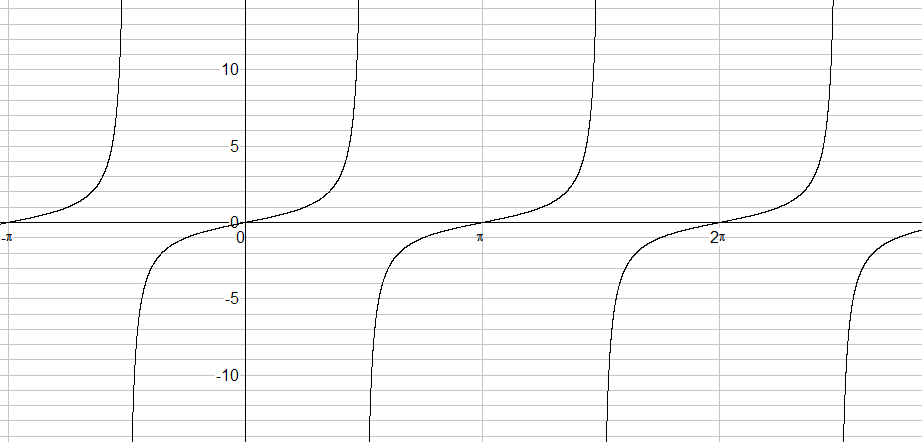
\includegraphics[ width=5.9646in, height=2.8772in,]{L4SZ270M}
}


The graph can be seen to have point symmetry. \ If you rotate the tangent curve through
a half turn using the origin as axis the curve will lie on top of itself. \ This is a pictorial representation
of an odd function.

Aside: You must not confuse $y =\tan  x$ with $y =x^{3}$. \ While they may appear to be similar in shape the only similarities are that they both
pass through the origin and continue towards $\infty $ in the first quadrant and $ -\infty $ in the third quadrant. \ Important differences that you should identify if you
are asked to sketch these graphs are the slope of the curves at the origin and the behaviour as $y \leadsto  \pm \infty $. 


\begin{tabular}[c]{l|l|l|}  & $y =x^{3}$  & $y =\tan  x$  \\
\hline
Slope of the curve at the origin  & $m =0$ {\scriptsize (horizontal)}  & $m =1$  \\
\hline
As $y \leadsto \infty $  & As $x \leadsto \infty $ $y \leadsto \infty $  & As $x \leadsto \frac{\pi }{2}$ $y \leadsto \infty $  \\
\hline
As $y \leadsto  -\infty $  & As $x \leadsto  -\infty $ $y \leadsto  -\infty $  & As $x \leadsto  -\frac{\pi }{2}$ $y \leadsto  -\infty $  \\
\hline
Asymptotes  & No
asymptotes  & Every $\left (2 n -1\right ) \frac{\pi }{2}$ $\left ( \forall n \in \mathbb{Z}\right )$  \\
\hline
Periodicity
& No period  & Period $ =\pi $  \\
\hline
Domain  & $\mathbb{R}$  & $\mathbb{R}$ except $\left (2 n -1\right ) \frac{\pi }{2}$  \\
\hline
\end{tabular}

\subsection{Transformations}
The six transformations that we reviewed in section 7.3 apply also to the tangent function. 

\subsubsection{Example}
(a) $y =\tan  \left (x -2\right )$ shifts the tangent curve 2 to the right. 

(b) $y =\tan  x +2$ shifts the tangent curve 2 upwards. 

(c) $y =2 \tan  x$ is a vertical stretch of $2$. 

(d) $y =\tan  2 x$ is a horizontal stretch of $\frac{1}{2}$. 

(e) $y = -\tan  x$ is a reflection in the $x$-axis. 

(f) $y =\tan  \left ( -x\right )$ is a reflection in the $y$-axis. 

You could use Omnigraph to verify that these are correctly stated. 

$y =a \tan  k t$ where $a$ and $k$ are both $ >0$ represent a vertical stretch of $a$ and a horizontal stretch of $\frac{1}{k}$. \ This means that if the period of $y =\tan  t$ is $\pi $ then the period of $y =a \tan  k t$ is $\frac{\pi }{k}$. \ If $0 <a <1$ the transformation is a shrinking not a stretching. \ If $0 <k <1$ then $\frac{1}{k} >1$. \ The period (which is $\frac{\pi }{k} =\pi  \times \frac{1}{k}$) will be $ >\pi $. 

\subsection{Exercises}
The following exercises from p 452 - 453 have been covered in this section: 


\begin{description}
\item [1.] A point $P ( -\frac{\sqrt{3}}{2} ,\frac{1}{2})$ is given. \ (a) Show that $P$ lies on the unit circle. \ (b) Suppose that $P$ is the terminal point determined by $t$. \ Find $\sin  t$, $\cos  t$ and $\tan  t\text{.}$ 

\item [3.] Given $t =\frac{2 \pi }{3}\text{.}$ Find the terminal point $P (x ,y)$ on the unit circle determined by $t$ and find $\sin  t$, $\cos  t$ and $\tan  t\text{.}$ \end{description}

Find the values of the trigonometric ratios.
\ If possible give the exact value; otherwise use a calculator to find an approximate value correct to 5 decimal
places. 


\begin{description}
\item [9.]   
%TCIMACRO{\TeXButton{Start Two Columns}{\columnsep =30pt
% \begin {multicols}{2}}}%
%BeginExpansion
\columnsep =30pt
\begin {multicols}{2}
%EndExpansion
 (a) $\sin  1.1\text{\quad \quad }$(b) $\cos  1.1$ 

\item [10.] (a) $\cos  \frac{\pi }{5}\text{\quad \quad }$(b) $\cos  \left ( -\frac{\pi }{5}\right )$ 
%TCIMACRO{\TeXButton{End Two Columns}{\end {multicols}}}%
%BeginExpansion
\end {multicols}
%EndExpansion
 

\item [21.]
Given $\sin  t =\frac{5}{13}$ and $\cos  t = -\frac{12}{13}$ find $\tan  t$ \end{description}

\section{Answers}
\textbf{Exercises 2.1} 

\begin {multicols}{2}

5. $P \left (\frac{4}{5} ,\frac{3}{5}\right )$ 

7. $P \left (\frac{ -\sqrt{5}}{3} ,\frac{2}{3}\right )$ 

9. $P \left (\frac{ -\sqrt{2}}{3} ,\frac{ -\sqrt{7}}{3}\right )$ 

13. $\left (0 ,1\right )$ 

15. $\left (\frac{ -\sqrt{3}}{2} ,\frac{1}{2}\right )$ 

17. $\left (\frac{1}{2} ,\frac{ -\sqrt{3}}{2}\right )$ 

19. $\left ( -\frac{1}{2} ,\frac{\sqrt{3}}{2}\right )$ 

21. $\left (\frac{ -\sqrt{2}}{2} ,\frac{ -\sqrt{2}}{2}\right )$ 

23. (a) $\left ( -\frac{3}{5} ,\frac{4}{5}\right )$, (b) $\left (\frac{3}{5} , -\frac{4}{5}\right )$ (c) $\left ( -\frac{3}{5} , -\frac{4}{5}\right )$  \\\relax (d)
$\left ( -\frac{3}{5} , -\frac{4}{5}\right )$ 

\end{multicols}

\textbf{Exercises 2.2} 
\begin{multicols}{2}

3.
(a) $\frac{ -\sqrt{3}}{2}$ (b) $\frac{1}{2}$ 

5. (a) $ -1$ (b) $ -1$ 

7. (a) $1$ (b) $ -1$ 

9. (a) $0$ (b) $0$ 

13. (a) $\frac{1}{2}$ (b) $\frac{1}{2}$ 

15. (a) $\frac{\sqrt{3}}{3}$ (b) $\frac{ -\sqrt{3}}{3}$ 

27. $\frac{4}{5} ,\frac{3}{5} ,\frac{4}{3}$ 

29. $\frac{ -\sqrt{11}}{4} ,\frac{\sqrt{5}}{4} ,\frac{ -\sqrt{55}}{5}$ 

35. $0.84147$ 

37. $0.93204$ 

39. $1.02964$ 

41. $ -0.57482\vspace{+5.000000cm}$ 
\end{multicols}
\clearpage

\textbf{Exercises 2.3} 
\begin{multicols}{2}

\begin{tabular}[c]{ll}1.  &
\setlength\fboxrule{0.01in}\setlength\fboxsep{0.2in}\fcolorbox[HTML]{000000}{FFFFFF}{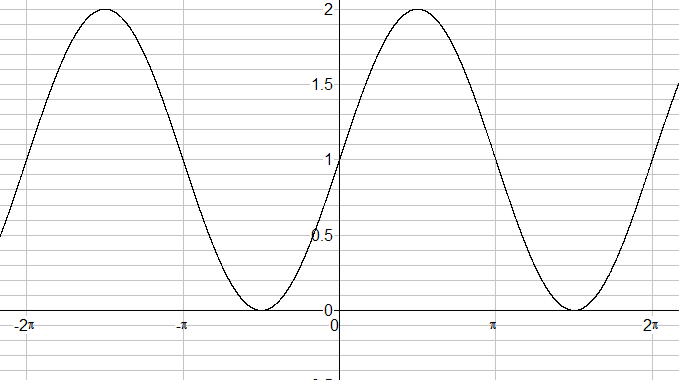
\includegraphics[ width=1.7115in, height=0.9625in,]{L4SZ270N}
}
\vspace{0.5cm}  \\
3.  &
\setlength\fboxrule{0.01in}\setlength\fboxsep{0.2in}\fcolorbox[HTML]{000000}{FFFFFF}{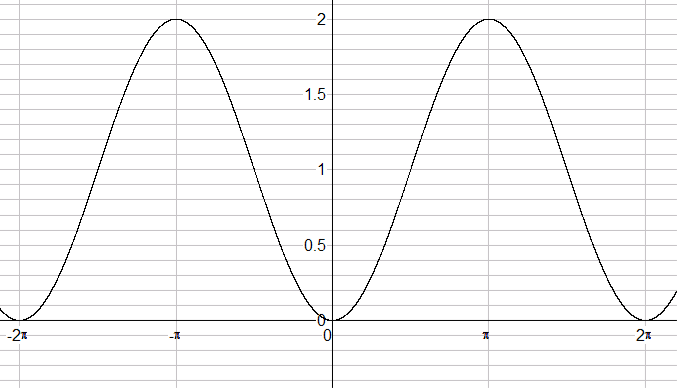
\includegraphics[ width=1.7279in, height=0.9945in,]{L4SZ270O}
}
\vspace{0.5cm}  \\
5.  &
\setlength\fboxrule{0.01in}\setlength\fboxsep{0.2in}\fcolorbox[HTML]{000000}{FFFFFF}{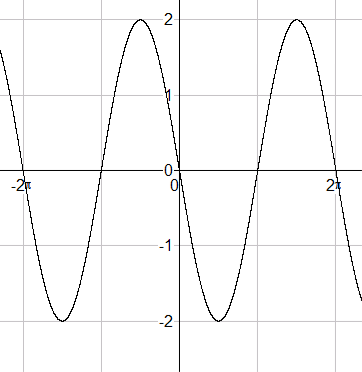
\includegraphics[ width=1.7253in, height=1.7737in,]{L4SZ270P}
}
\vspace{0.5cm}  \\
7.  &
\setlength\fboxrule{0.01in}\setlength\fboxsep{0.2in}\fcolorbox[HTML]{000000}{FFFFFF}{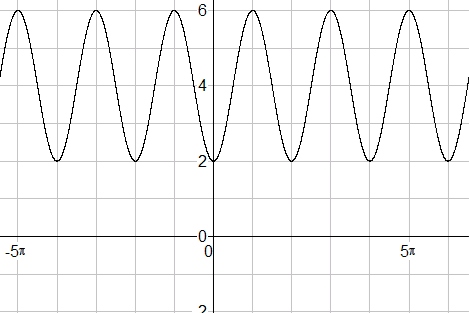
\includegraphics[ width=1.753in, height=1.1727in,]{L4SZ270Q}
}
\vspace{0.5cm}  \\
9.  &
\setlength\fboxrule{0.01in}\setlength\fboxsep{0.2in}\fcolorbox[HTML]{000000}{FFFFFF}{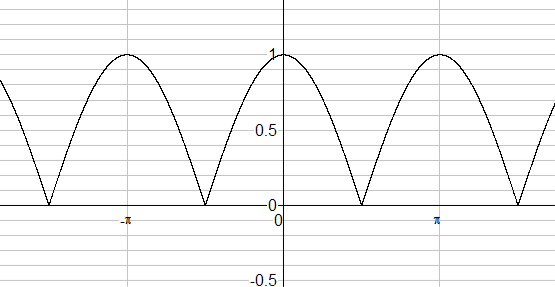
\includegraphics[ width=1.7642in, height=0.9167in,]{L4SZ270R}
}
\vspace{0.5cm}
\end{tabular}


\begin{tabular}[c]{ll}11.  & $1 ,\frac{\pi }{2}$  \\
 &    
\setlength\fboxrule{0.01in}\setlength\fboxsep{0.2in}\fcolorbox[HTML]{000000}{FFFFFF}{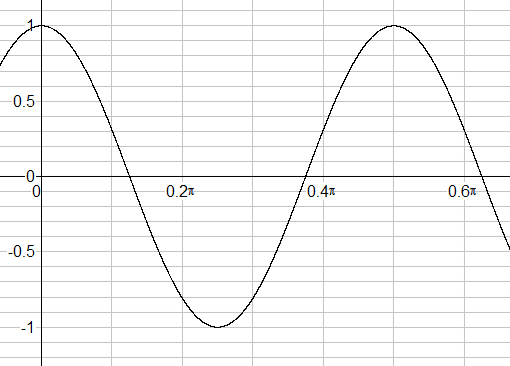
\includegraphics[ width=1.9666in, height=1.4157in,]{L4SZ270S}
}
\end{tabular}


\begin{tabular}[c]{ll}13.  & $3 ,\frac{2 \pi }{3}$  \\
 &    
\setlength\fboxrule{0.01in}\setlength\fboxsep{0.2in}\fcolorbox[HTML]{000000}{FFFFFF}{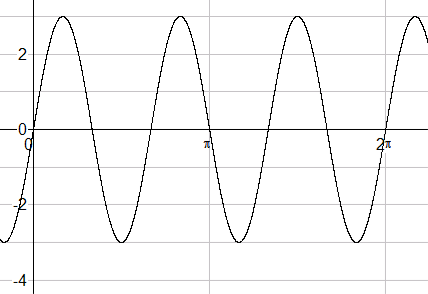
\includegraphics[ width=1.9692in, height=1.3569in,]{L4SZ270T}
}
\end{tabular}


\begin{tabular}[c]{ll}15.  & $10 ,4 \pi $  \\
 &    
\setlength\fboxrule{0.01in}\setlength\fboxsep{0.2in}\fcolorbox[HTML]{000000}{FFFFFF}{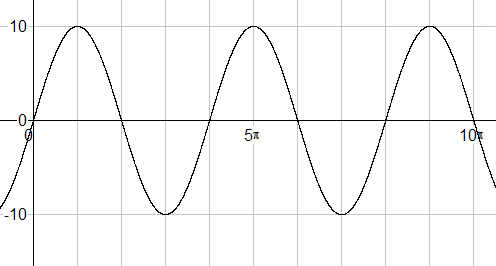
\includegraphics[ width=2.1802in, height=1.1744in,]{L4SZ270U}
}
\end{tabular}


\begin{tabular}[c]{ll}17.  & $1 ,6 \pi $  \\
 &    
\setlength\fboxrule{0.01in}\setlength\fboxsep{0.2in}\fcolorbox[HTML]{000000}{FFFFFF}{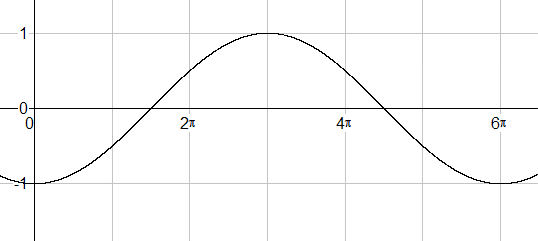
\includegraphics[ width=2.3013in, height=1.036in,]{L4SZ270V}
}
\end{tabular}


\begin{tabular}[c]{ll}19.  & $3 ,\frac{2}{3}$ note the non-trig scale  \\
 &
\setlength\fboxrule{0.01in}\setlength\fboxsep{0.2in}\fcolorbox[HTML]{000000}{FFFFFF}{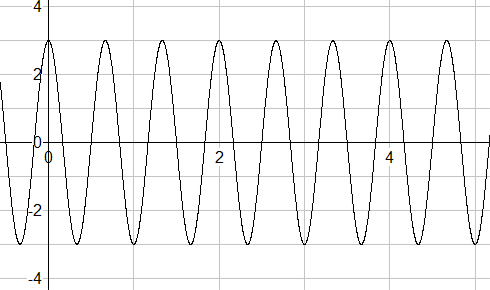
\includegraphics[ width=2.4933in, height=1.4806in,]{L4SZ270W}
}
\end{tabular}


\begin{tabular}[c]{ll}21.  & $1 ,2 \pi  ,\frac{\pi }{2}$  \\
 &    
\setlength\fboxrule{0.01in}\setlength\fboxsep{0.2in}\fcolorbox[HTML]{000000}{FFFFFF}{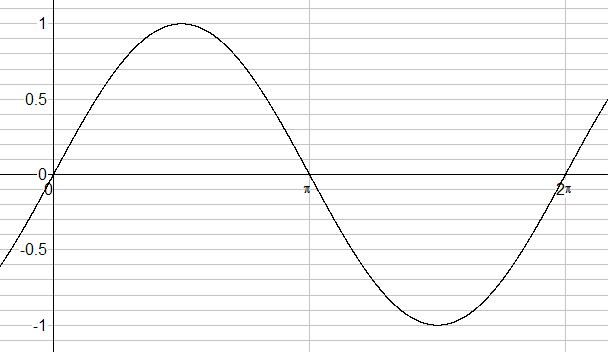
\includegraphics[ width=2.4794in, height=1.4416in,]{L4SZ270X}
}
\end{tabular}


\begin{tabular}[c]{ll}23.  & $2 ,2 \pi  ,\frac{\pi }{6}$  \\
 &    
\setlength\fboxrule{0.01in}\setlength\fboxsep{0.2in}\fcolorbox[HTML]{000000}{FFFFFF}{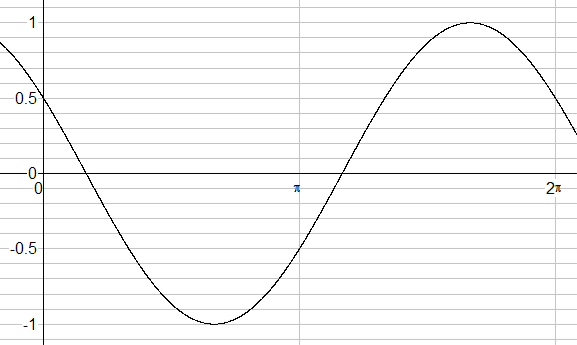
\includegraphics[ width=2.4794in, height=1.4883in,]{L4SZ270Y}
}
\end{tabular}


\begin{tabular}[c]{ll}25.  & $5 ,\frac{2 \pi }{3} ,\frac{\pi }{12}$  \\
 &    
\setlength\fboxrule{0.01in}\setlength\fboxsep{0.2in}\fcolorbox[HTML]{000000}{FFFFFF}{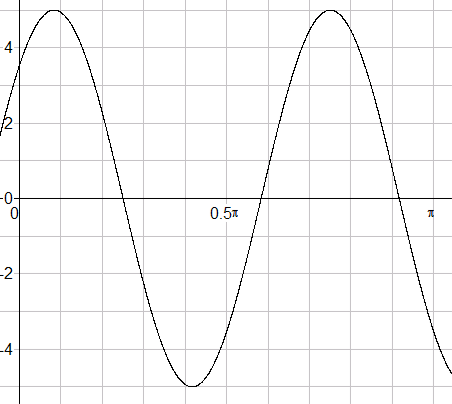
\includegraphics[ width=2.1724in, height=1.9441in,]{L4SZ270Z}
}
\end{tabular}


\begin{tabular}[c]{ll}27.  & $2 ,3 \pi  ,\frac{\pi }{4}$  \\
 &    
\setlength\fboxrule{0.01in}\setlength\fboxsep{0.2in}\fcolorbox[HTML]{000000}{FFFFFF}{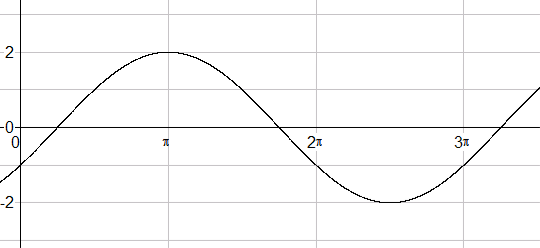
\includegraphics[ width=2.4336in, height=1.1243in,]{L4SZ2710}
}
\end{tabular}


\begin{tabular}[c]{ll}29.  & $3 ,2 , -\frac{1}{2}$  \\
 &    
\setlength\fboxrule{0.01in}\setlength\fboxsep{0.2in}\fcolorbox[HTML]{000000}{FFFFFF}{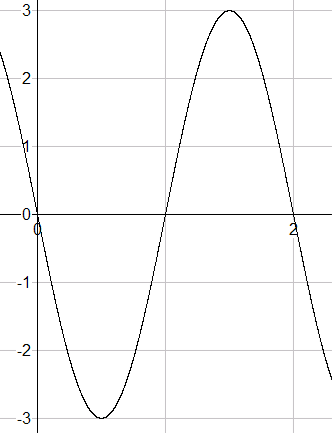
\includegraphics[ width=2.1543in, height=1.8498in,]{L4SZ2711}
}
\end{tabular}


\begin{tabular}[c]{ll}31.  & $\frac{1}{2} ,\pi  ,\frac{\pi }{6}$  \\
 &    
\setlength\fboxrule{0.01in}\setlength\fboxsep{0.2in}\fcolorbox[HTML]{000000}{FFFFFF}{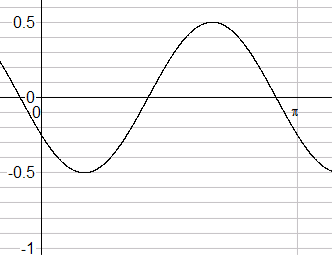
\includegraphics[ width=1.9216in, height=1.4797in,]{L4SZ2712}
}
\end{tabular}


\begin{tabular}[c]{ll}33.  & $1 ,\frac{2 \pi }{3} , -\frac{\pi }{3}$  \\
 &    
\setlength\fboxrule{0.01in}\setlength\fboxsep{0.2in}\fcolorbox[HTML]{000000}{FFFFFF}{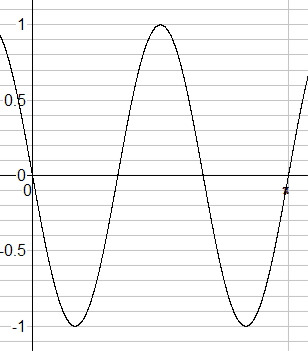
\includegraphics[ width=1.4408in, height=1.6397in,]{L4SZ2713}
}
\end{tabular}


\begin{tabular}[c]{ll}41.  &  \\
 &
\setlength\fboxrule{0.01in}\setlength\fboxsep{0.2in}\fcolorbox[HTML]{000000}{FFFFFF}{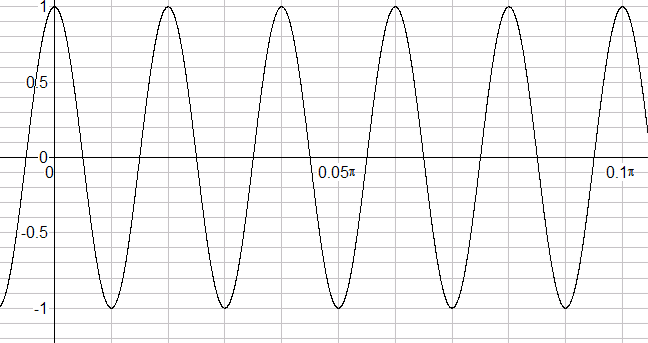
\includegraphics[ width=2.3168in, height=1.2315in,]{L4SZ2714}
}
\end{tabular}


\begin{tabular}[c]{ll}43.  &  \\
 &
\setlength\fboxrule{0.01in}\setlength\fboxsep{0.2in}\fcolorbox[HTML]{000000}{FFFFFF}{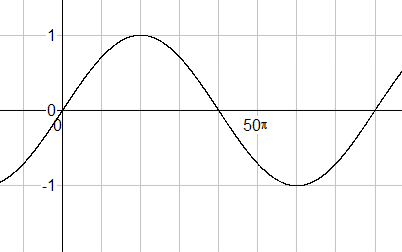
\includegraphics[ width=2.0989in, height=1.3214in,]{L4SZ2715}
}
\end{tabular}


\begin{tabular}[c]{ll}47.  &  \\
 &
\setlength\fboxrule{0.01in}\setlength\fboxsep{0.2in}\fcolorbox[HTML]{000000}{FFFFFF}{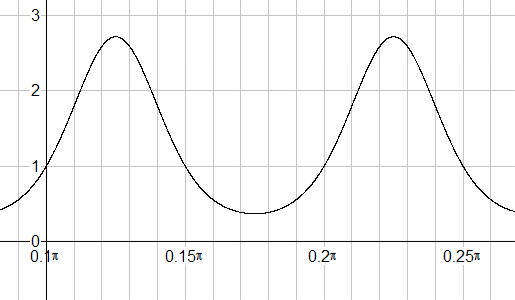
\includegraphics[ width=2.3722in, height=1.3872in,]{L4SZ2816}
}
\end{tabular}


\begin{tabular}[c]{ll}53.  &  \\
 &
\setlength\fboxrule{0.01in}\setlength\fboxsep{0.2in}\fcolorbox[HTML]{000000}{FFFFFF}{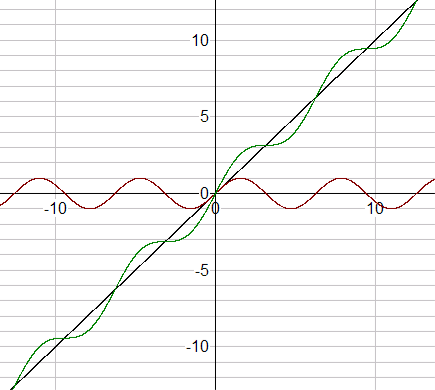
\includegraphics[ width=2.4621in, height=2.2096in,]{L4SZ2817}
}
\end{tabular}


\begin{tabular}[c]{ll}55.  &  \\
 &
\setlength\fboxrule{0.01in}\setlength\fboxsep{0.2in}\fcolorbox[HTML]{000000}{FFFFFF}{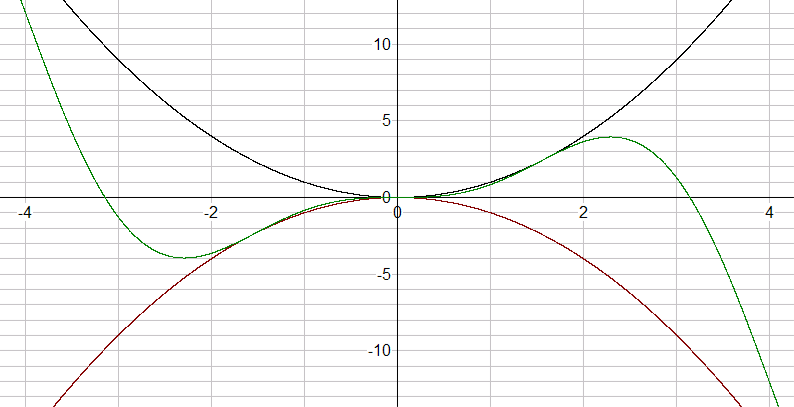
\includegraphics[ width=2.5399in, height=1.3085in,]{L4SZ2818}
}
\end{tabular}


\begin{tabular}[c]{ll}57.  &  \\
 &
\setlength\fboxrule{0.01in}\setlength\fboxsep{0.2in}\fcolorbox[HTML]{000000}{FFFFFF}{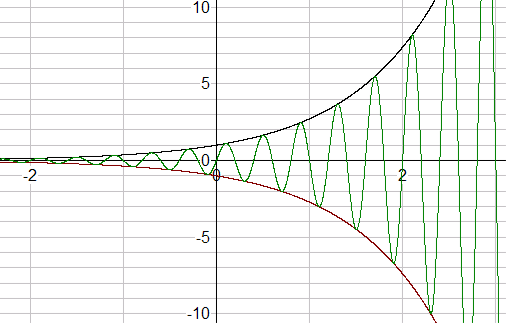
\includegraphics[ width=2.5564in, height=1.6371in,]{L4SZ2819}
}
\end{tabular}
\end{multicols}

61. Maximum value $1.76$ when $x \approx 0.94$, minimum value $ -1.76$ when $x \approx  -0.94\text{.}$ \ The same maximum and minimum values occur at infinitely many other values
of $x$. 

63. Maximum value $3.00$ when $x \approx 1.57\text{,}$ minimum value $ -1.00$ when $x \approx  -1.57$. The same maximum and minimum values occur at infinitely many other values of $x$. 

65. $1.16$ 

\textbf{Exercises 2.4} 
\begin{multicols}{2}

1. (b) $\frac{1}{2} ,\frac{ -\sqrt{3}}{2} ,\frac{ -\sqrt{3}}{3}$ 

3. $\left ( -\frac{1}{2} ,\frac{\sqrt{3}}{2}\right ) ,\sin  t =\frac{\sqrt{3}}{2} ,\cos  t = -\frac{1}{2} ,\tan  t = -\sqrt{3}$ 

9. (a) $0.89121$ (b) $0.45360$ 

10. (a) $0.80902$ (b) $0.80902$ 

21. $ -\frac{5}{12}$ 
\end{multicols}
